\documentclass[journal,10pt,twocolumn]{IEEEtran}
\usepackage{graphicx}
\usepackage[margin=0.5in]{geometry}
\usepackage[cmex10]{amsmath}
\usepackage{amssymb}
\usepackage{array}
\usepackage{booktabs}
\usepackage{mathtools}
\usepackage{dirtree}
\usepackage{xcolor}
\usepackage{float}
\usepackage[justification=centering,font={rm,md,scriptsize}]{caption}
\usepackage{enumitem}
\usepackage{listings}
\usepackage{mathtools}
\usepackage{fancyvrb}
%\usepackage{hyperref}


%Add chapter functionality in IEEEtran class
\newcounter{Chapcounter}
\newcommand\showmycounter{\addtocounter{Chapcounter}{1}\themycounter}
\newcommand{\chapter}[1] 
{ {\centering          
  \addtocounter{Chapcounter}{1} \large \textbf{Chapter \theChapcounter ~#1}}  
  \addcontentsline{toc}{section}{Chapter ~\theChapcounter~~ #1}    
  \setcounter{section}{0}
}
%%%%

\counterwithin{enumi}{section}
\counterwithin{equation}{enumi}
\counterwithin{figure}{enumi}

\renewcommand\thesection{\theChapcounter.\arabic{section}}
\renewcommand\thesectiondis{\theChapcounter.\arabic{section}}
\newcommand\figref{Fig.~\ref}

\setenumerate{label=\thesection.\arabic*}

\lstset{
  basicstyle=\ttfamily,
  columns=fullflexible,
  frame=single,
  breaklines=true,
  postbreak=\mbox{\textcolor{red}{$\hookrightarrow$}\space},
}

\providecommand{\mbf}{\mathbf}
\providecommand{\pr}[1]{\ensuremath{\Pr\left(#1\right)}}
\providecommand{\qfunc}[1]{\ensuremath{Q\left(#1\right)}}
\providecommand{\sbrak}[1]{\ensuremath{{}\left[#1\right]}}
\providecommand{\lsbrak}[1]{\ensuremath{{}\left[#1\right.}}
\providecommand{\rsbrak}[1]{\ensuremath{{}\left.#1\right]}}
\providecommand{\brak}[1]{\ensuremath{\left(#1\right)}}
\providecommand{\lbrak}[1]{\ensuremath{\left(#1\right.}}
\providecommand{\rbrak}[1]{\ensuremath{\left.#1\right)}}
\providecommand{\cbrak}[1]{\ensuremath{\left\{#1\right\}}}
\providecommand{\lcbrak}[1]{\ensuremath{\left\{#1\right.}}
\providecommand{\rcbrak}[1]{\ensuremath{\left.#1\right\}}}
\newcommand{\sgn}{\mathop{\mathrm{sgn}}}
\providecommand{\abs}[1]{\left\vert#1\right\vert}
\providecommand{\res}[1]{\Res\displaylimits_{#1}} 
\providecommand{\norm}[1]{\left\lVert#1\right\rVert}
\providecommand{\mtx}[1]{\mathbf{#1}}
\providecommand{\mean}[1]{E\left[ #1 \right]}
\providecommand{\fourier}{\overset{\mathcal{F}}{ \rightleftharpoons}}
\providecommand{\ztrans}{\overset{\mathcal{Z}}{ \rightleftharpoons}}
\providecommand{\system}{\overset{\mathcal{H}}{ \longleftrightarrow}}
\newcommand{\solution}{\noindent \textbf{Solution: }}
\newcommand{\cosec}{\,\text{cosec}\,}
\providecommand{\dec}[2]{\ensuremath{\overset{#1}{\underset{#2}{\gtrless}}}}
\newcommand{\myvec}[1]{\ensuremath{\begin{pmatrix}#1\end{pmatrix}}}
\newcommand{\mydet}[1]{\ensuremath{\begin{vmatrix}#1\end{vmatrix}}}
\providecommand{\gauss}[2]{\mathcal{N}\ensuremath{\left(#1,#2\right)}}
\newcommand*{\permcomb}[4][0mu]{{{}^{#3}\mkern#1#2_{#4}}}
\newcommand*{\perm}[1][-3mu]{\permcomb[#1]{P}}
\newcommand*{\comb}[1][-1mu]{\permcomb[#1]{C}}

\let\vec\mathbf

\def\putbox#1#2#3{\makebox[0in][l]{\makebox[#1][l]{}\raisebox{\baselineskip}[0in][0in]{\raisebox{#2}[0in][0in]{#3}}}}
     \def\rightbox#1{\makebox[0in][r]{#1}}
     \def\centbox#1{\makebox[0in]{#1}}
     \def\topbox#1{\raisebox{-\baselineskip}[0in][0in]{#1}}
     \def\midbox#1{\raisebox{-0.5\baselineskip}[0in][0in]{#1}}

\begin{document}

\title{Module 2 Digital Communication}
\author{Mannava Venkatasai}
\date{December 2022}

\maketitle
\bigskip

\chapter{Two Dice}
\section{Sum of Independant Random Variables}
Two dice, one blue and one grey, are thrown at the same time.   The event defined by the sum of the two numbers appearing on the top of the dice can have 11 possible outcomes 2, 3, 4, 5, 6, 7, 8, 9, 10, 11 and 12.  A student argues that each of these outcomes has a probability $\frac{1}{11}$.  Do you agree with this argument?  Justify your answer.
%

\begin{enumerate}
\item  {\em The Uniform Distribution: }Let $X_i \in \cbrak{1,2,3,4,5,6}, i = 1,2,$ be the random variables representing the outcome for each die.  Assuming the dice to be fair, the probability mass function (pmf) is expressed as 
\begin{align}
\label{eq:dice_pmf_xi}
p_{X_i}(n) = \pr{X_i = n} = 
\begin{cases}
\frac{1}{6} & 1 \le n \le 6
\\
0 & otherwise
\end{cases}
\end{align}
The desired outcome is
\begin{align}
\label{eq:dice_xdef}
X &= X_1 + X_2,
\\
\implies X &\in \cbrak{1,2,\dots,12}
\end{align}
%
The objective is to show that
\begin{align}
p_X(n) \ne \frac{1}{11}
\label{eq:dice_wrong}
\end{align}
\item {\em Convolution: }
From \eqref{eq:dice_xdef},
\begin{align}
p_X(n) &= \pr{X_1 + X_2 = n} = \pr{X_1  = n -X_2}
\\
&= \sum_{k}^{}\pr{X_1  = n -k | X_2 = k}p_{X_2}(k)
\label{eq:dice_x_sum}
\end{align}%
after unconditioning.  $\because X_1$ and $X_2$ are independent,
\begin{multline}
\pr{X_1  = n -k | X_2 = k} 
\\
= \pr{X_1  = n -k} = p_{X_1}(n-k)
\label{eq:dice_x1_indep}
\end{multline}
From \eqref{eq:dice_x_sum} and \eqref{eq:dice_x1_indep},
\begin{align}
p_X(n) = \sum_{k}^{}p_{X_1}(n-k)p_{X_2}(k) = p_{X_1}(n)*p_{X_2}(n)
\label{eq:dice_x_conv}
\end{align}
where $*$ denotes the convolution operation. 
%\cite{proakis_dsp}.  
Substituting from \eqref{eq:dice_pmf_xi}
in \eqref{eq:dice_x_conv},
\begin{align}
p_X(n) = \frac{1}{6}\sum_{k=1}^{6}p_{X_1}(n-k)= \frac{1}{6}\sum_{k=n-6}^{n-1}p_{X_1}(k)
\label{eq:dice_x_conv_x1}
\end{align}
\begin{align}
\because p_{X_1}(k) &= 0, \quad k \le 1, k \ge 6.
\end{align}
From \eqref{eq:dice_x_conv_x1},
%
\begin{align}
p_X(n) &= 
\begin{cases}
0 & n < 1
\\
\frac{1}{6}\sum_{k=1}^{n-1}p_{X_1}(k) &  1 \le n-1 \le  6
\\
\frac{1}{6}\sum_{k=n-6}^{6}p_{X_1}(k) & 1 < n-6 \le 6
\\
0 & n > 12
\end{cases}
\label{eq:dice_x_conv_cond}
\end{align}
Substituting from \eqref{eq:dice_pmf_xi} in \eqref{eq:dice_x_conv_cond},
\begin{align}
p_X(n) &= 
\begin{cases}
0 & n < 1
\\
\frac{n-1}{36} &  2 \le n \le  7
\\
\frac{13-n}{36} & 7 < n \le 12
\\
0 & n > 12
\end{cases}
\label{eq:dice_x_conv_final}
\end{align}
satisfying \eqref{eq:dice_wrong}.
\item {\em The $Z$-transform: }
The $Z$-transform of $p_X(n)$ is defined as 
%\cite{proakis_dsp}
\begin{align}
P_X(z) = \sum_{n = -\infty}^{\infty}p_X(n)z^{-n}, \quad z \in \mathbb{C}
\label{eq:dice_xz}
\end{align}
%
From \eqref{eq:dice_pmf_xi} and \eqref{eq:dice_xz}, 
\begin{align}
P_{X_1}(z) =P_{X_2}(z) &= \frac{1}{6}\sum_{n = 1}^{6}z^{-n}
\\
&=\frac{z^{-1}\brak{1-z^{-6}}}{6\brak{1-z^{-1}}}, \quad \abs{z} > 1
\label{eq:dice_xiz}
\end{align}
upon summing up the geometric progression.  
\begin{align}
\because p_X(n) &= p_{X_1}(n)*p_{X_2}(n),
\\
P_X(z) &= P_{X_1}(z)P_{X_2}(z)
\label{eq:dice_xzprod_def}
\end{align}
The above property follows from Fourier analysis and is fundamental to signal processing. 
%\cite{proakis_dsp}. 
From \eqref{eq:dice_xiz} and \eqref{eq:dice_xzprod_def},
\begin{align}
P_X(z) &= \cbrak{\frac{z^{-1}\brak{1-z^{-6}}}{6\brak{1-z^{-1}}}}^2
\\
&= \frac{1}{36}\frac{z^{-2}\brak{1-2z^{-6}+z^{-12}}}{\brak{1-z^{-1}}^2}
\label{eq:dice_xzprod}
\end{align}
Using the fact that 
%\cite{proakis_dsp}
\begin{align}
p_X(n-k) &\system{Z}P_X(z)z^{-k},
\\
nu(n)&\system{Z} \frac{z^{-1}}{\brak{1-z^{-1}}^2}
\end{align}
after some algebra, it can be shown that
%{\tiny
\begin{multline}
\frac{1}{36}\lsbrak{\brak{n-1}u(n-1) - 2 \brak{n-7}u(n-7)}
\\
\rsbrak{ +\brak{n-13}u(n-13)}
\\
\system{Z}
\frac{1}{36}\frac{z^{-2}\brak{1-2z^{-6}+z^{-12}}}{\brak{1-z^{-1}}^2}
\label{eq:dice_xz_closed}
\end{multline}
%}

where 
\begin{align}
u(n) =
\begin{cases}
1 & n \ge 0
\\
0 & n < 0
\end{cases}
\end{align}

From \eqref{eq:dice_xz}, \eqref{eq:dice_xzprod} and \eqref{eq:dice_xz_closed}
\begin{multline}
p_{X}(n) = \frac{1}{36}\lsbrak{\brak{n-1}u(n-1) 
}
\\
\rsbrak{- 2 \brak{n-7}u(n-7)+\brak{n-13}u(n-13)}
\end{multline}
which is the same as \eqref{eq:dice_x_conv_final}.  Note that  \eqref{eq:dice_x_conv_final} can be obtained from \eqref{eq:dice_xz_closed} using contour integration as well.
% \cite{proakis_dsp}.  

\item 
The experiment of rolling the dice was simulated using Python for 10000 samples.  These were generated using Python libraries for uniform distribution. The frequencies for each outcome were then used to compute the resulting pmf, which  is plotted in Figure \ref{fig:dice}.  The theoretical pmf obtained in \eqref{eq:dice_x_conv_final} is plotted for comparison.  
%
\begin{figure}[H]
\centering
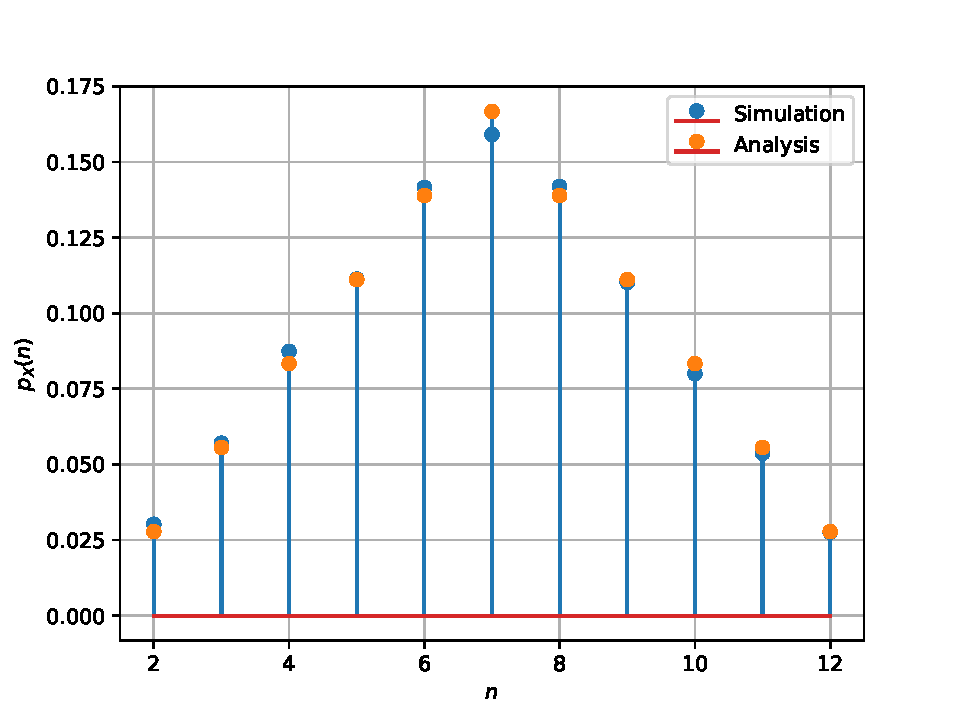
\includegraphics[width=\columnwidth]{./pmf_dice.pdf}
\caption{Plot of $p_X(n)$.  Simulations are close to the analysis. }
\label{fig:dice}
\end{figure}
\item The python code is available in 
\begin{lstlisting}
	https://github.com/Mannava123455/module_2/blob/main/probability/codes/chapter_1/1.py
\end{lstlisting}
\end{enumerate}




\chapter{Random Numbers}
\section{Uniform Random Numbers}
Let $U$ be a uniform random variable between 0 and 1.
\begin{enumerate}
\item Generate $10^6$ samples of $U$ using a C program and save into a file called uni.dat .
\label{prob:uni_gen}
\\
\solution Download the following files and execute the  C program.
\begin{lstlisting}
	https://github.com/Mannava123455/module_2/blob/main/probability/codes/chapter_2/2_1_1.c
\end{lstlisting}

%
\item
Load the uni.dat file into python and plot the empirical CDF of $U$ using the samples in uni.dat. The CDF is defined as
\begin{align}
F_{U}(x) = \pr{U \le x}
\end{align}

\begin{lstlisting}
	https://github.com/Mannava123455/module_2/blob/main/probability/codes/chapter_2/2_1_1_cdfplot.py
\end{lstlisting}
\begin{figure}[H]
\centering
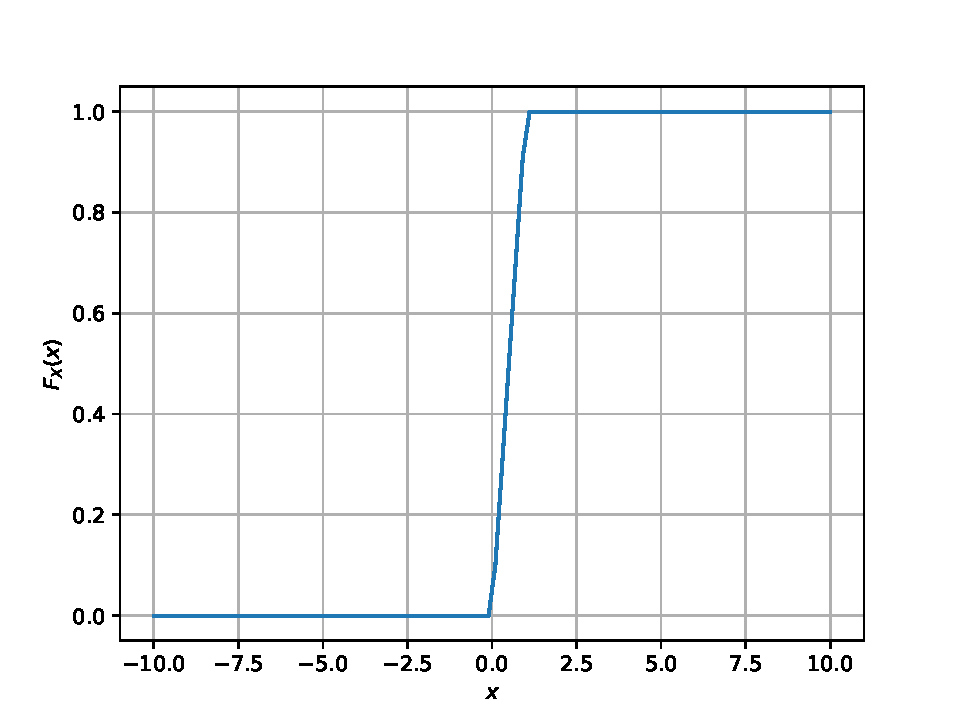
\includegraphics[width=\columnwidth]{./uni_cdf.pdf}
\caption{The CDF of $U$}
\label{fig:uni_cdf}
\end{figure}
\item
Find a  theoretical expression for $F_{U}(x)$.\\
\solution
\begin{align} 
F_{U}(x) = \int_{-\infty}^{x} f_{U}(x)\,dx
\label{eq:pdf_to_cdf}
\end{align}
For the uniform random variable $U$, $f_{U}(x)$ is given by  
\begin{align}
	f_U(x) &= 
	\begin{cases}
	1 &  0 \le x \le  1
	\\
	0 & elsewhere
	\\
	\end{cases}
	\label{eq:uni_pdf}
\end{align}
Substituting \eqref{eq:uni_pdf} in \eqref{eq:pdf_to_cdf}, $F_U(x)$ is found to be
\begin{align}
	F_U(x) &= 
	\begin{cases}
	0 & x < 0
	\\	
	x & 0 \le x \le  1
	\\
	1 & x > 0
	\\
	\end{cases}
	\label{eq:uni_cdf}
\end{align}

\item
\label{prob:print_uni}
The mean of $U$ is defined as
%
\begin{equation}
E\sbrak{U} = \frac{1}{N}\sum_{i=1}^{N}U_i
\end{equation}
%
and its variance as
%
\begin{equation}
\text{var}\sbrak{U} = E\sbrak{U- E\sbrak{U}}^2 
\end{equation}

Write a C program to  find the mean and variance of $U$.\\
\solution The following code prints the mean and variance of $U$
\begin{lstlisting}
	https://github.com/Mannava123455/module_2/blob/main/probability/codes/chapter_2/2_1_1.c
\end{lstlisting}
The output of the program is
\begin{lstlisting}
Uniform stats:
Mean: 0.500007
Variance: 0.083301
\end{lstlisting}

\item Verify your result theoretically given that
%
\begin{equation}
E\sbrak{U^k} = \int_{-\infty}^{\infty}x^kdF_{U}(x)
\end{equation}\\
\solution For a random variable $X$, the mean $\mu_X$ and variance $\sigma_X^2$ are given by
\begin{align}
	\label{eq:mean_exp}
	\mu_X &= E\sbrak{X} = \int_{-\infty}^{\infty}xdF_{U}(x) \\
	\label{eq:var_exp}
	\sigma_X^2 &= E\sbrak{X^2} - \mu_X^2 = \int_{-\infty}^{\infty}x^2dF_{U}(x) - \mu_X^2
\end{align}  
Substituting the CDF of $U$ from (2.1.3.3) in (2.1.5.2) and (2.1.5.3), we get
\begin{align}
	\label{eq:mean_uni}
	\mu_U &= \frac{1}{2} \\
	\label{eq:var_uni}
	\sigma_U^2 &= \frac{1}{12}
\end{align}  
which match with the values printed in problem 2.1.4
\end{enumerate}


\section{Central Limit Theorem}
\begin{enumerate}
%
%
\item
Generate $10^6$ samples of the random variable
%
\begin{equation}
X = \sum_{i=1}^{12}U_i -6
\end{equation}
%
using a C program, where $U_i, i = 1,2,\dots, 12$ are  a set of independent uniform random variables between 0 and 1
and save in a file called gau.dat\\
\solution Download the following files and execute the  C program.
\begin{lstlisting}
	https://github.com/Mannava123455/module_2/blob/main/probability/codes/chapter_2/2_2.c
\end{lstlisting}
%
\item
Load gau.dat in python and plot the empirical CDF of $X$ using the samples in gau.dat. What properties does a CDF have?
\\
\begin{figure}[H]
\centering
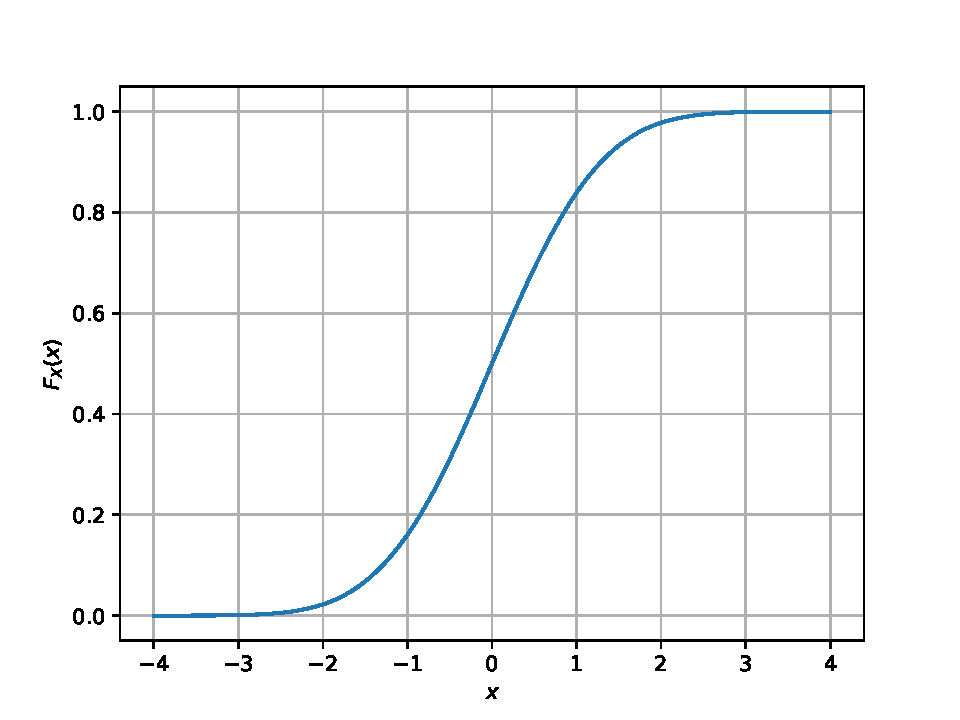
\includegraphics[width=\columnwidth]{gauss_cdf.pdf}
\caption{The CDF of $X$}
\label{fig:gauss_cdf}
\end{figure}
The properties of a CDF are
\begin{eqnarray}
	F_X(-\infty) = 0\\
	F_X(\infty) = 1\\
	\frac{dF_X(x)}{dx} \ge 0
\end{eqnarray}
\item
Load gau.dat in python and plot the empirical PDF of $X$ using the samples in gau.dat. The PDF of $X$ is defined as
\begin{align}
p_{X}(x) = \frac{d}{dx}F_{X}(x)
\label{eq:cdf_to_pdf}
\end{align}
What properties does the PDF have?
\\
\solution 
\begin{lstlisting}
	https://github.com/Mannava123455/module_2/blob/main/probability/codes/chapter_2/2_2_pdf.py
\end{lstlisting}

\begin{figure}[H]
\centering
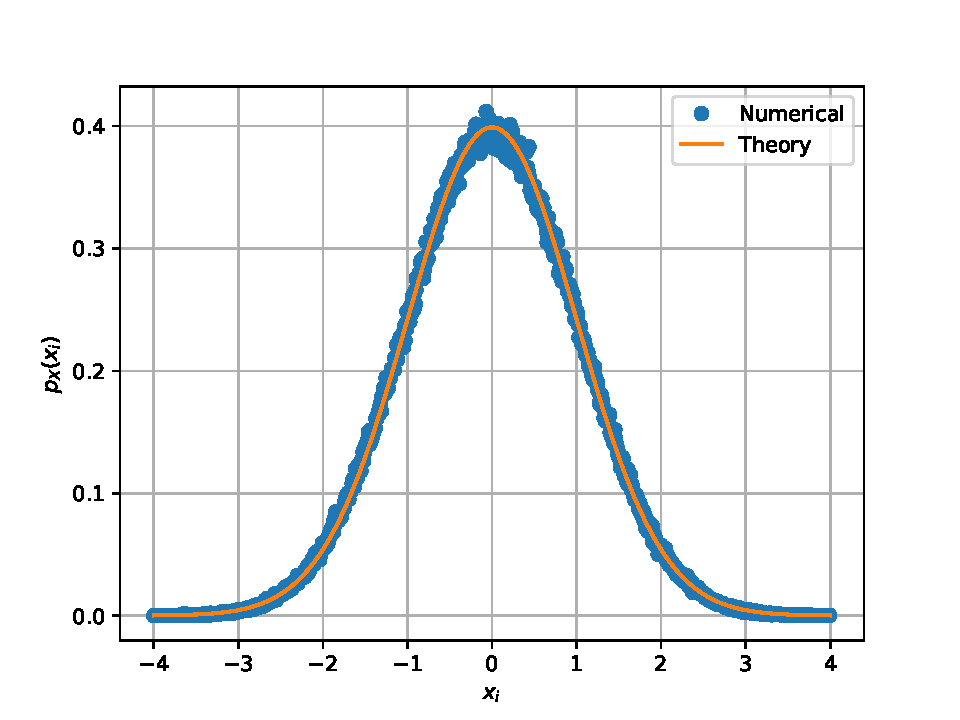
\includegraphics[width=\columnwidth]{gauss_pdf.pdf}
\caption{The PDF of $X$}
\label{fig:gauss_pdf}
\end{figure}

The properties of PDF are
\begin{eqnarray}
	f_X(x) \ge 0\\
	\int_{-\infty}^{\infty} f_X(x) \,dx = 1
\end{eqnarray}

\item Find the mean and variance of $X$ by writing a C program.
\solution The following code prints the mean and variance of $X$
\begin{lstlisting}
	https://github.com/Mannava123455/module_2/blob/main/probability/codes/chapter_2/2_2_mean.c
\end{lstlisting}
The output of the program is
\begin{lstlisting}
Gaussian stats:
Mean: 0.000294
Variance: 0.999562	
\end{lstlisting}
\item Given that 
\begin{align}
p_{X}(x) = \frac{1}{\sqrt{2\pi}}\exp\brak{-\frac{x^2}{2}}, -\infty < x < \infty,
\label{eq:gau_pdf}
\end{align}
repeat the above exercise theoretically.\\
\solution Substituting the PDF from \eqref{eq:gau_pdf} in \eqref{eq:mean_exp},
\begin{flalign}
	\mu_X &= \int_{-\infty}^{\infty} \frac{x}{\sqrt{2\pi}}\exp\brak{-\frac{x^2}{2}} \,dx&\\
	\intertext{Using}&\\
	\int x \cdot \exp \left( -a x^2 \right) \mathrm{d}x &= -\frac{1}{2a} \cdot \exp \left( -a x^2 \right)&\\
	\mu_X &= \frac{1}{\sqrt{2\pi}}\left[-\exp\brak{-\frac{x^2}{2}}\right]_{-\infty}^{\infty}&\\  
	\mu_X &= 0
\end{flalign}
Substituting $\mu_X$ and the PDF in \eqref{eq:var_exp} to compute variance,
\begin{flalign}
	\sigma_X^2 &= \int_{-\infty}^{\infty} \frac{x^2}{\sqrt{2\pi}}\exp\brak{-\frac{x^2}{2}} \,dx&\\ \nonumber
	\intertext{Substituting} t &= \frac{x^2}{2},&\\	
	\sigma_X^2 &= \frac{2}{\sqrt{\pi}} \int_{0}^{\infty} t^{\frac{1}{2}}\exp\brak{-t} \,dt&\\	\nonumber
	&= \frac{2}{\sqrt{\pi}} \int_{0}^{\infty} t^{\frac{3}{2}-1}\exp\brak{-t} \,dt&\\
	\intertext{Using the gamma function} \Gamma(x) &= \int_{0}^{\infty} z^{x-1} \cdot e^{-z} \, \mathrm{d}z \,&\\
	\sigma_X^2 &= \frac{2}{\sqrt{\pi}}\Gamma(\frac{3}{2})&\\	\nonumber
	&= \frac{2}{\sqrt{\pi}}\frac{\sqrt{\pi}}{2}&\\	\nonumber
	&=1	
\end{flalign}
%
\end{enumerate}


\section{From Uniform to Other}
\begin{enumerate}
%
\item
Generate samples of 
%
\begin{equation}
V = -2\ln\brak{1-U}
\end{equation}
%
and plot its CDF. \\
\solution
\begin{lstlisting}
	https://github.com/Mannava123455/module_2/blob/main/probability/codes/chapter_2/2_3.c
\end{lstlisting}
\begin{lstlisting}
	https://github.com/Mannava123455/module_2/blob/main/probability/codes/chapter_2/2_3_cdf.py
\end{lstlisting}
\begin{figure}[H]
\centering
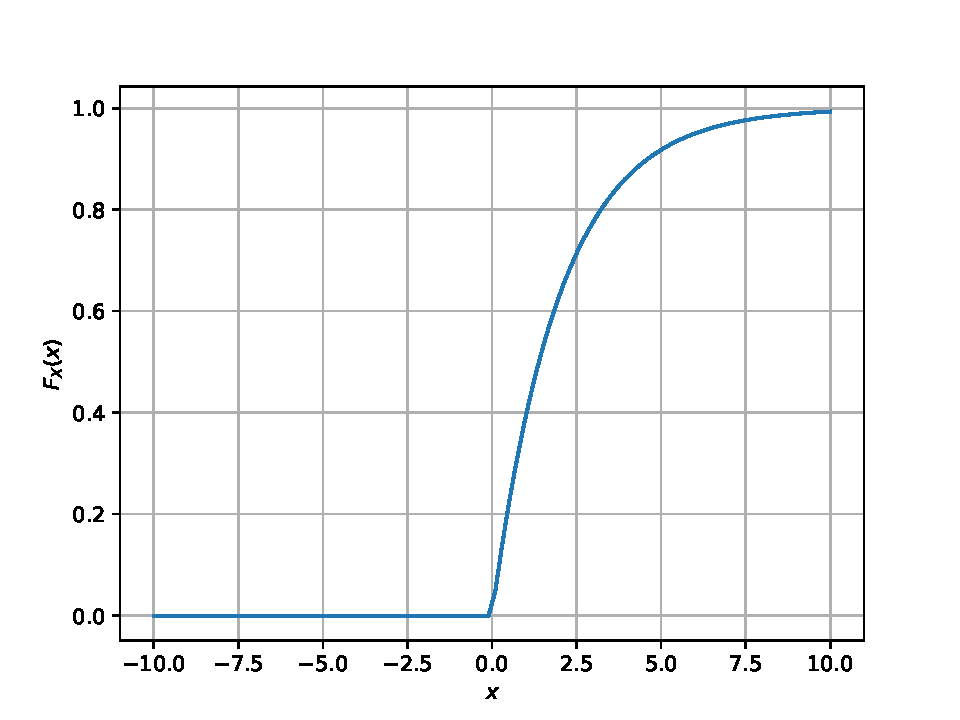
\includegraphics[width=\columnwidth]{log.pdf}
\caption{The CDF of $V$}
\label{fig:log_uni_cdf}
\end{figure}
\item Find a theoretical expression for $F_V(x)$.
\begin{flalign}
	F_V(x) &= P(V < x)&\\
	&= P(-2\ln\brak{1-U} < x)&\\
	&= P(U < 1 - e^{\frac{-x}{2}})&\\
	&= F_U(1 - e^{\frac{-x}{2}})
\end{flalign}
Using $F_U(x)$ defined in \eqref{eq:uni_cdf},
\begin{align}
	F_V(x) &=
	\begin{cases}
		0 & x < 0\\
		1 - e^{\frac{-x}{2}} & x \ge 0
	\end{cases}
\end{align} 
\end{enumerate}



\section{Triangular Distribution}
%
\begin{enumerate}
\item Generate 
	\begin{align}
		T = U_1+U_2
	\end{align}\\
\solution Download the following files and execute the  C program.
\begin{lstlisting}
	https://github.com/Mannava123455/module_2/blob/main/probability/codes/chapter_2/triangle.c
\end{lstlisting}
\item Find the CDF of $T$.\\
\solution 
\begin{lstlisting}
	https://github.com/Mannava123455/module_2/blob/main/probability/codes/chapter_2/2.4.5_cdf.py
\end{lstlisting}
\begin{figure}[H]
\centering
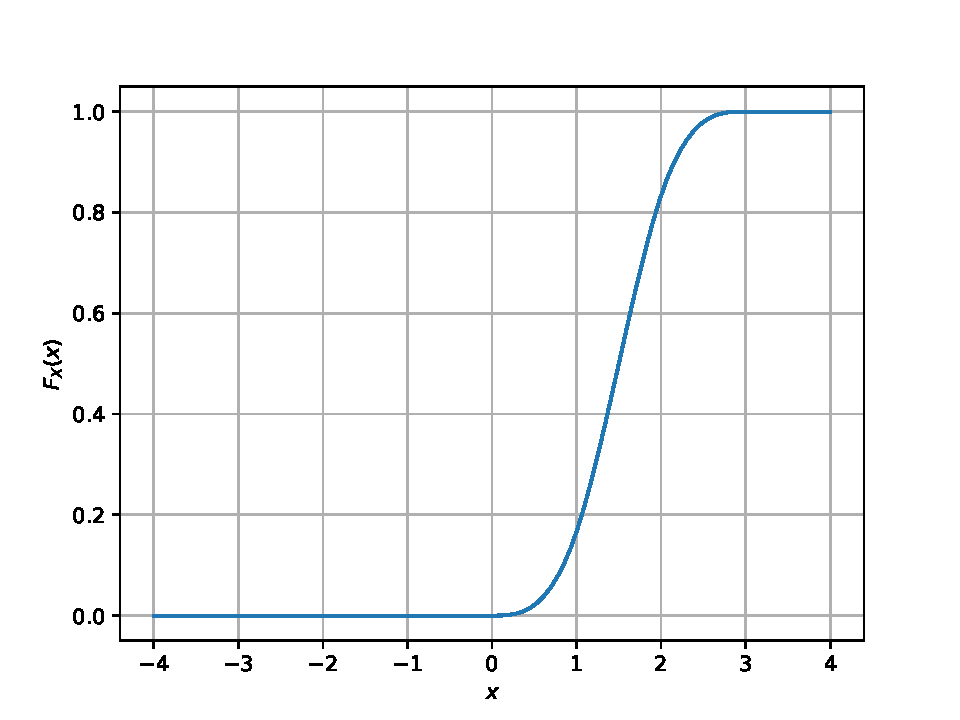
\includegraphics[width=\columnwidth]{triangle_cdf.pdf}
\caption{The CDF of $T$}
\label{fig:tri_cdf}
\end{figure}
\item Find the PDF of $T$.\\

\begin{lstlisting}
	https://github.com/Mannava123455/module_2/blob/main/probability/codes/chapter_2/2.4.5_pdf.py
\end{lstlisting}
\begin{figure}[H]
\centering
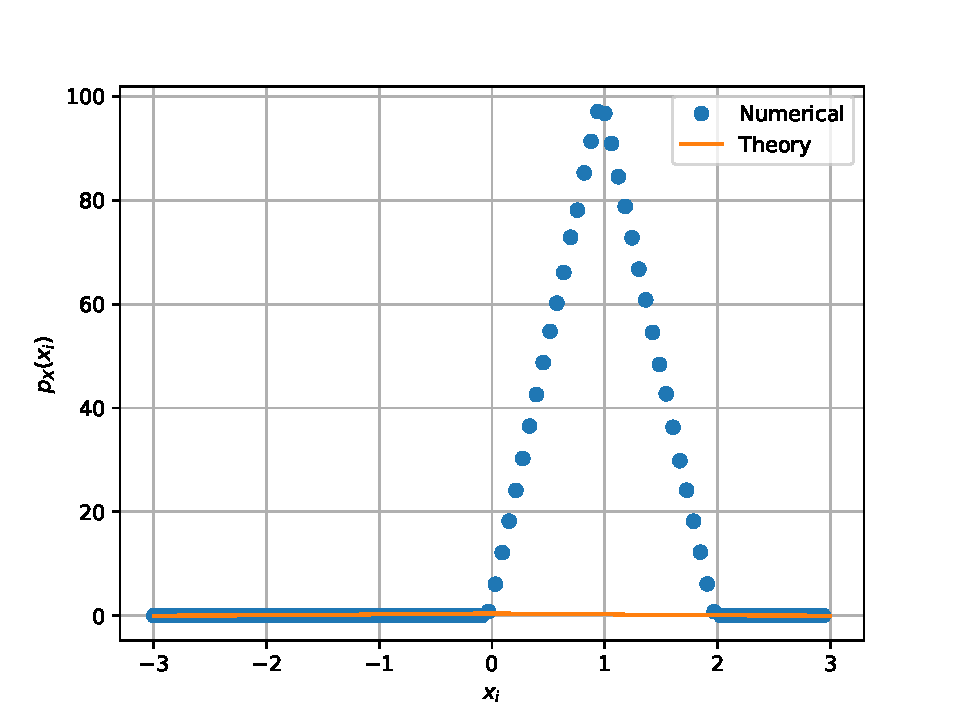
\includegraphics[width=\columnwidth]{triangle_pdf.pdf}
\caption{The PDF of $T$}
\label{fig:tri_pdf}
\end{figure}
\item Find the theoretical expressions for the PDF and CDF of $T$.\\
\solution Since $T$ is the sum of two independant random variables $U1$ and $U2$, the PDF of $T$ is given by
\begin{flalign}
	p_T(x) &= p_{U1}(x) \ast p_{U2}(x)
\end{flalign}
Using the PDF of $U$ from \eqref{eq:uni_pdf}, the convolution results in
\begin{align}
	p_T(x) &=
	\begin{cases}
		0 & x < 0\\
		x & 0 \le x \le 1\\
		2-x & 1 \le x \le 2\\
		0 & x > 2
	\end{cases}
	\label{eq:tri_pdf}
\end{align}
The CDF of $T$ is found using \eqref{eq:pdf_to_cdf} by replacing $U$ with $T$. Evaluating the integral for the piecewise function $p_T(x)$, 
\begin{align}
	F_T(x) &=
	\begin{cases}
		0 & x < 0\\
		\frac{x^2}{2} & 0 \le x \le 1\\
		2x-\frac{x^2}{2}-1 & 1 \le x \le 2\\
		1 & x > 2
	\end{cases}
\end{align}
\item Verify your results through a plot. \\
\solution 
\end{enumerate}
\vspace{100mm}
\chapter{Maximum Likelihood Detection: BPSK}
\section{Maximum Likelihood}
\begin{enumerate}
\item Generate equiprobable $X \in \cbrak{1,-1}$.\\
\solution $X$ can be generated in python using the below code section,

\item Generate 
\begin{equation}
Y = AX+N,
\end{equation}
where $A = 5$ dB,  and $N \sim \gauss{0}{1}$.\\
\solution $Y$ can be generated in python using the below code section,
\begin{lstlisting}
	https://github.com/Mannava123455/module_2/blob/main/probability/codes/chapter_3/3_1.py
\end{lstlisting}
\item Plot $Y$ using a scatter plot.\\
\solution 
\begin{lstlisting}
	https://github.com/Mannava123455/module_2/blob/main/probability/codes/chapter_3/3_1.py
\end{lstlisting}
\begin{figure}[H]
\centering
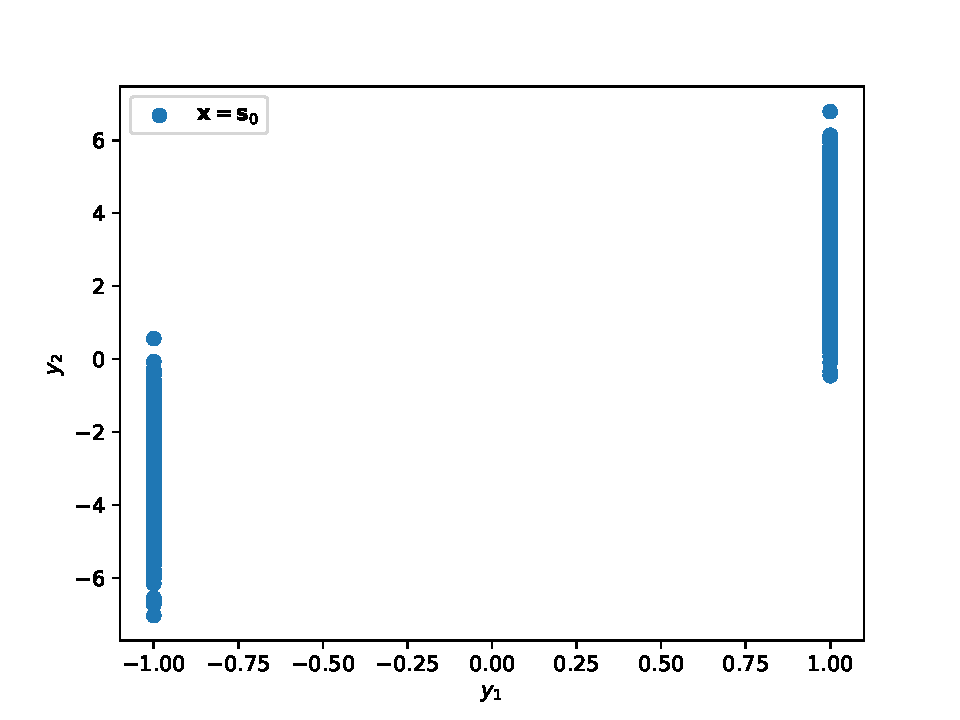
\includegraphics[width=\columnwidth]{/home/mannava/latex/3.pdf}
\caption{Scatter plot of $Y$}
\label{fig:bpsk_scatter}
\end{figure}
\item Guess how to estimate $X$ from $Y$.\\
\solution
\begin{equation}
y \dec{1}{-1} 0
\label{eq:bpsk_decision}
\end{equation}
\item
\label{ml-ch4_sim}
Find 
\begin{equation}
	P_{e|0} = \pr{\hat{X} = -1|X=1}
\end{equation}
and 
\begin{equation}
	P_{e|1} = \pr{\hat{X} = 1|X=-1}
\end{equation}\\
\solution
\begin{flalign*}
	\pr{\hat{X} = -1|X=1} &= \pr{Y < 0|X=1}&\\
	&= \pr{AX + N < 0|X=1}&\\ 
	&= \pr{A + N < 0}&\\
	&= \pr{N < -A}
\end{flalign*}
Similarly,
\begin{flalign*}
	\pr{\hat{X} = 1|X=-1} &= \pr{Y > 0|X=-1}&\\
	&= \pr{N > A}
\end{flalign*}
Since $N \sim \gauss{0}{1}$,
\begin{flalign}
	\label{eq:std_norm_symmetric}
	\pr{N < -A} &= \pr{N > A}&\\
	\label{eq:bpks_prob_err_cond}
	\implies P_{e|0} &= P_{e|1} = \pr{N > A}
\end{flalign}
%
\item Find $P_e$ assuming that $X$ has equiprobable symbols.\\
\solution
\begin{flalign}
	P_e &= \pr{X=1}P_{e|1} + \pr{X=-1}P_{e|0}&\\
	\intertext{Since $X$ is equiprobable}\\
	\label{eq:bpsk_prob_error_equi}
	P_e &= \frac{1}{2}P_{e|1} + \frac{1}{2}P_{e|0}
\end{flalign}
Substituting from \eqref{eq:bpks_prob_err_cond}
\begin{equation}
	P_e = \pr{N > A}
\end{equation}
Given a random varible $X \sim \gauss{0}{1}$ the Q-function is defined as
\begin{align}
	Q(x) &= \pr{X > x}\\
	\label{eq:q_func_integral}
	Q(x) &= \frac{1}{\sqrt{2\pi}} \int_x^\infty \exp\left(-\frac{u^2}{2}\right) \, du.\\
\end{align}
Using the Q-function, $P_e$ is rewritten as
\begin{equation}
	P_e = Q(A)
\end{equation} 
%
\item
Verify by plotting  the theoretical $P_e$ with respect to $A$ from 0 to 10 dB.\\
\solution 
\begin{lstlisting}
	https://github.com/Mannava123455/module_2/blob/main/probability/codes/chapter_3/3.1.7.py
\end{lstlisting}
\begin{figure}[H]
\centering
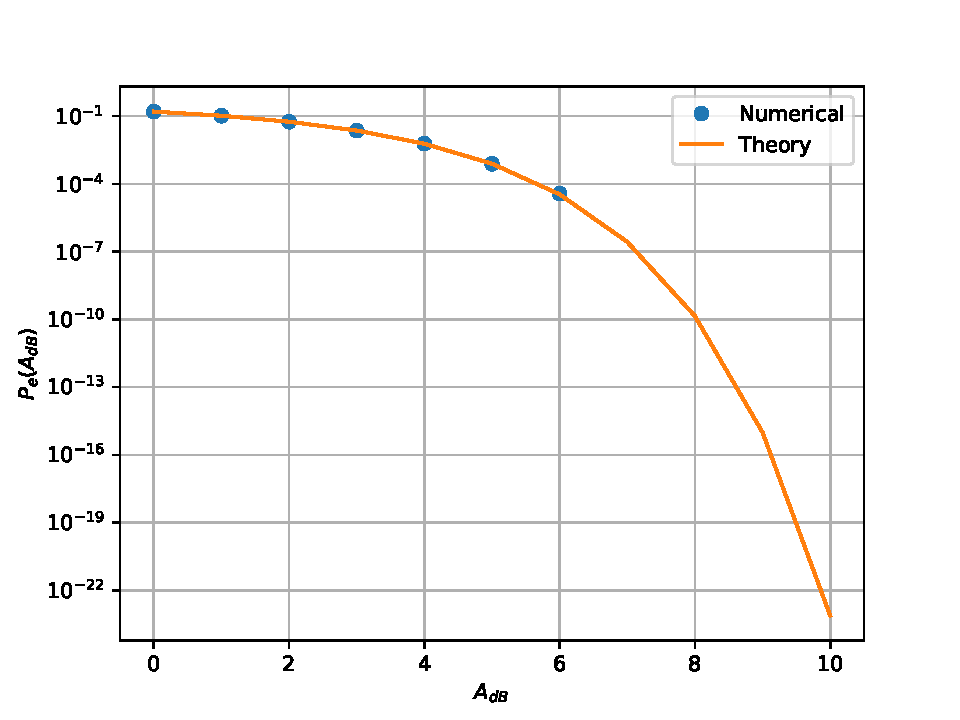
\includegraphics[width=\columnwidth]{/home/mannava/latex/bpsk_pe_snr.pdf}
\caption{$P_e$ versus $A$ plot}
\label{fig:bpsk_pe_snr}
\end{figure}
%
\item Now, consider a threshold $\delta$  while estimating $X$ from $Y$. Find the value of $\delta$ that maximizes the theoretical $P_e$.\\
\label{prob:bpsk_delta_equi}
\solution Given the decision rule, 
\begin{equation}
y \dec{1}{-1} \delta
\label{eq:bpsk_decision_delta}
\end{equation}
\begin{flalign*}
	P_{e|0} &= \pr{\hat{X} = -1|X=1}&\\
	&= \pr{Y < \delta|X=1}&\\
	&= \pr{AX + N < \delta|X=1}&\\ 
	&= \pr{A + N < \delta}&\\
	&= \pr{N < -A + \delta}&\\
	&= \pr{N > A - \delta}&\\
	&= Q(A-\delta)
\end{flalign*}
\begin{flalign*}
	P_{e|1} &= \pr{\hat{X} = 1|X=-1}&\\
	&= \pr{Y > \delta|X=-1}&\\
	&= \pr{N > A + \delta}&\\
	&= Q(A+\delta)
\end{flalign*}
Using \eqref{eq:bpsk_prob_error_equi}, $P_e$ is given by
\begin{flalign}
	P_e &= \frac{1}{2}Q(A+\delta) + \frac{1}{2}Q(A-\delta)
\end{flalign}
Using the integral for Q-function from \eqref{eq:q_func_integral},
\begin{align}
	\label{eq:prob_error_delta_equi}
	P_e &= k(\int_{A+\delta}^\infty \exp\left(-\frac{u^2}{2}\right) \, du + \int_{A-\delta}^\infty \exp\left(-\frac{u^2}{2}\right) \, du)\\
	\intertext{where k is a constant}	\nonumber
\end{align}
Differentiating \eqref{eq:prob_error_delta_equi} wrt $\delta$ (using Leibniz's rule) and equating to $0$, we get
\begin{flalign*}
	\exp\left(-\frac{(A+\delta)^2}{2}\right)-\exp\left(-\frac{(A-\delta)^2}{2}\right) &= 0&\\
	\frac{\exp\left(-\frac{(A+\delta)^2}{2}\right)}{\exp\left(-\frac{(A-\delta)^2}{2}\right)} &= 1&\\
	\exp\left(-\frac{(A+\delta)^2-(A-\delta)^2}{2}\right) &= 1&\\
	\exp\left(-2A\delta\right) &= 1&\\
	\intertext{Taking $\ln$ on both sides}\\
	-2A\delta &= 0&\\
	\implies \delta &= 0
\end{flalign*}
$P_e$ is maximum for $\delta = 0$
\item Repeat the above exercise when 
\label{prob:bpsk_decision_uneqi}
	\begin{align}
		p_{X}(0) = p
	\end{align}\\
\solution Since $X$ is not equiprobable, $P_e$ is given by,
\begin{flalign}
	P_e &= (1-p)P_{e|1} + pP_{e|0}&\\
	&= (1-p)Q(A+\delta) + pQ(A-\delta)
\end{flalign}
Using the integral for Q-function from \eqref{eq:q_func_integral},
\begin{multline}
	\label{eq:prob_error_delta_nonequi}
	P_e = k((1-p)\int_{A+\delta}^\infty \exp\left(-\frac{u^2}{2}\right) \, du + \\
	p\int_{A-\delta}^\infty \exp\left(-\frac{u^2}{2}\right) \, du)
\end{multline}
where $k$ is a constant.\\
Following the same steps as in problem \ref{prob:bpsk_delta_equi}, $\delta$ for maximum $P_e$ evaluates to,
\begin{equation}
	\delta = \frac{1}{2A}\ln\left(\frac{1}{p}-1\right)
\end{equation}
\item Repeat the above exercise using the MAP criterion.\\
\solution 
The MAP rule can be stated as\\
\begin{flalign}
\label{eq:map_rule}
\text{Set } \hat{x} &= x_i \text{ if}&\\ \nonumber
p_X(x_k)p_Y(y|x_k) &\text{ is maximum for } k = i
\end{flalign}
For the case of BPSK, the point of equality between $p_X(x=1)p_Y(y|x=1)$ and $p_X(x=-1)p_Y(y|x=-1)$ is the optimum threshold. If this threshold is $\delta$, then
\begin{flalign*}
	pp_Y(y|x=1) > (1-p)p_Y(y|x=-1) &\text{ when } y > \delta&\\
	pp_Y(y|x=1) < (1-p)p_Y(y|x=-1) &\text{ when } y < \delta 	
\end{flalign*}
The above inequalities can be visualized in \figref{fig:bpsk_map_density} for $p = 0.3$ and $A = 3$.
\begin{figure}[H]
\centering
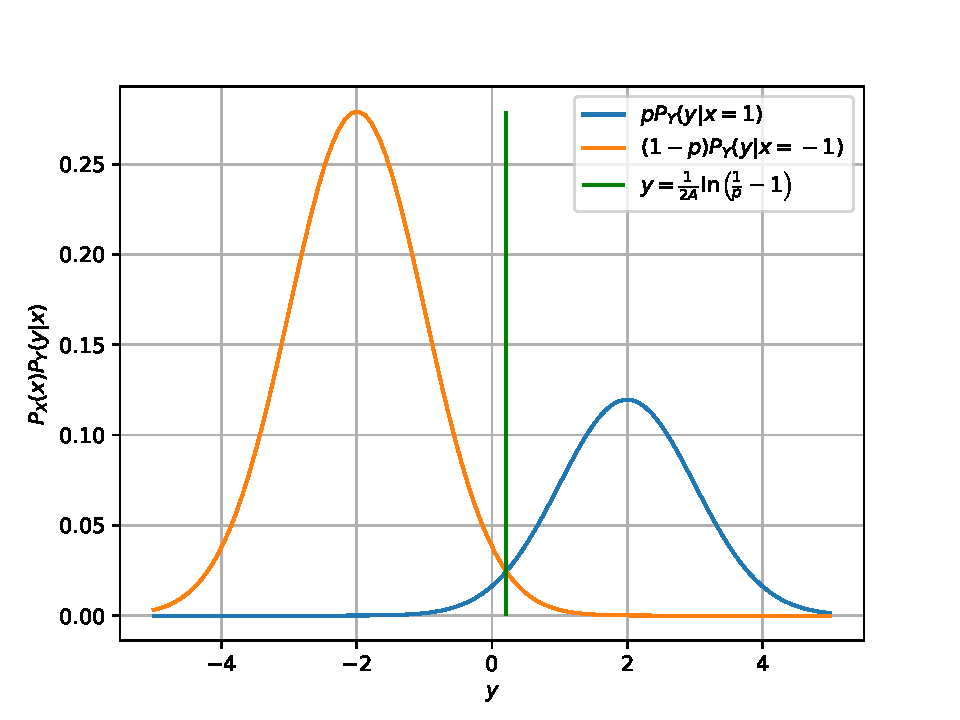
\includegraphics[width=\columnwidth]{/home/mannava/latex/bpsk_map_density.pdf}
\caption{$p_X(X=x_i)p_Y(y|x=x_i)$ versus $y$ plot for $X \in \{-1,1\}$}
\label{fig:bpsk_map_density}
\end{figure}
Given $Y=AX+N$ where $N \sim \gauss{0}{1}$, the optimum threshold is found as solution to the below equation
\begin{equation}
	p\exp\left(-\frac{(y_{eq}-A)^2}{2}\right) = (1-p)\exp\left(-\frac{(y_{eq}+A)^2}{2}\right)
\end{equation}
Solving for $y_{eq}$, we get
\begin{equation}S
	y_{eq} = \delta = \frac{1}{2A}\ln\left(\frac{1}{p}-1\right)
\end{equation}
which is same as $\delta$ obtained in problem \ref{prob:bpsk_decision_uneqi}

\begin{lstlisting}
	https://github.com/Mannava123455/module_2/blob/main/probability/codes/chapter_3/3_map.py
\end{lstlisting}
\end{enumerate}








\chapter{Transformation of Random Variables}
\section{Gaussian to Other}
\begin{enumerate}
\item
Let $X_1 \sim  \gauss{0}{1}$ and $X_2 \sim  \gauss{0}{1}$. Plot the CDF and PDF of
%
\begin{equation}
V = X_1^2 + X_2^2
\end{equation}\\
\solution The CDF and PDF of $V$ are plotted in \figref{fig:chisq_cdf} and \figref{fig:chisq_pdf} respectively using the below code
\begin{lstlisting}
	https://github.com/Mannava123455/module_2/blob/main/probability/codes/chapter_4/4_1_cdf.py

	https://github.com/Mannava123455/module_2/blob/main/probability/codes/chapter_4/4_1_pdf.py
\end{lstlisting}
\begin{figure}[H]
\centering
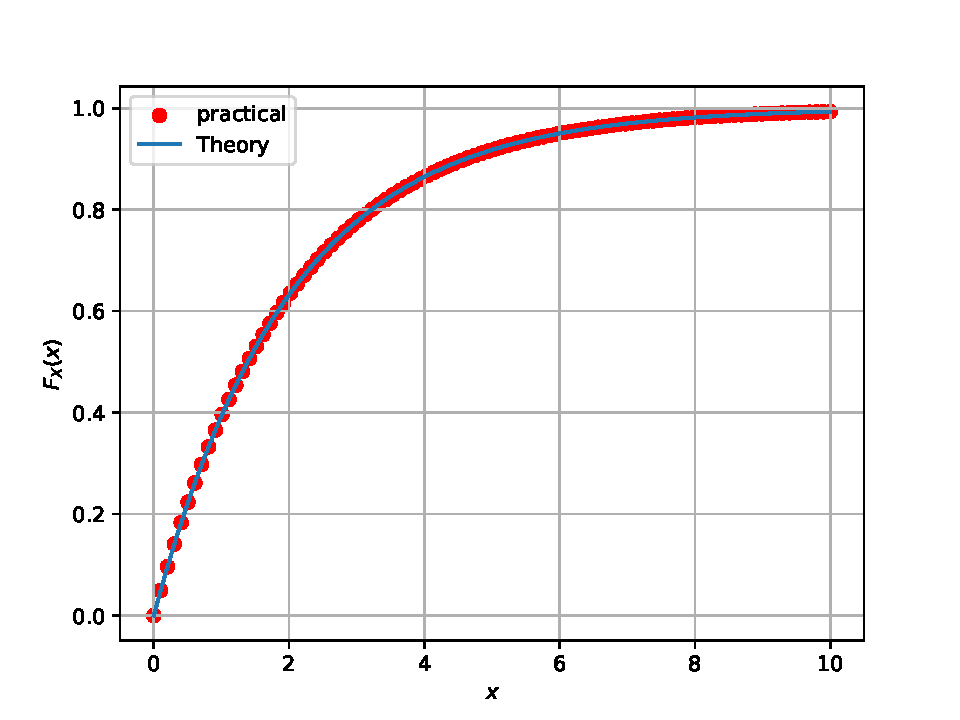
\includegraphics[width=\columnwidth]{/home/mannava/latex/chisq_cdf.pdf}
\caption{CDF of $V$}
\label{fig:chisq_cdf}
\end{figure}
\begin{figure}[H]
\centering
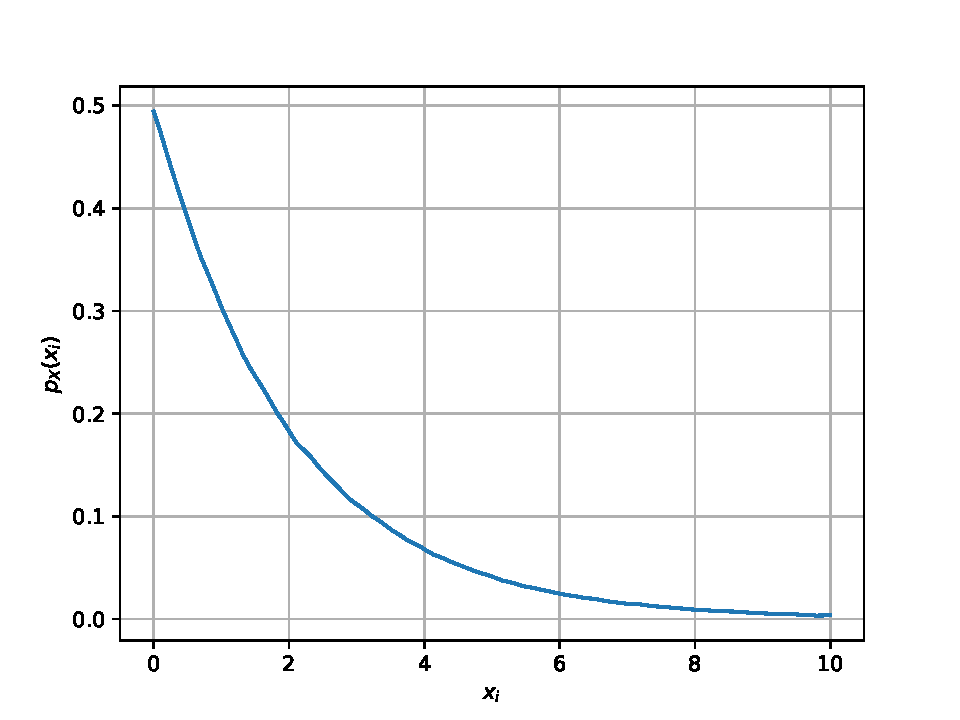
\includegraphics[width=\columnwidth]{/home/mannava/latex/pdf.pdf}
\caption{PDF of $V$}
\label{fig:chisq_pdf}
\end{figure}
%

%
%
\item
If
%
\begin{equation}
F_{V}(x) = 
\begin{cases}
1 - e^{-\alpha x} & x \geq 0 \\
0 & x < 0,
\end{cases}
\label{eq:chisq2_cdf_gen}
\end{equation}
%
find $\alpha$.\\
\solution Let $Z=X^2$ where $X \sim \gauss{0}{1}$. Defining the CDF for $Z$,
\begin{flalign*}
	P_Z(z) &= \pr{Z < z}&\\
	&= \pr{X^2 < z}&\\
	&= \pr{-\sqrt{z} < X < \sqrt{z}}&\\
	&= \int_{-\sqrt{z}}^{\sqrt{z}} p_X(x)  \,dx 
\end{flalign*}
Using \eqref{eq:cdf_to_pdf}, the PDF of $Z$ is given by
\begin{align}
	\nonumber
	\frac{d}{dz}P_Z(z) &= p_Z(z)\\
	\label{eq:square_pdf_gen}
	= \frac{p_X(\sqrt{z})+p_X(-\sqrt{z})}{2\sqrt{z}} & \text{ (Using Lebniz's rule)} 
\end{align}
Substituting the standard gaussian density function $p_X(x) = \frac{1}{\sqrt{2\pi}}e^{-\frac{x^2}{2}}$ in \eqref{eq:square_pdf_gen},
\begin{equation}
	p_Z(z) =
	\begin{cases}
	\frac{1}{\sqrt{2\pi z}}e^{-\frac{z}{2}} & z \ge 0\\
	0 & z < 0
	\end{cases} 
	\label{eq:chisq_pdf}
\end{equation}
The PDF of $X_1^2$ and $X_2^2$ are given by \eqref{eq:chisq_pdf}. Since $V$ is the sum of two independant random variables,
\begin{flalign*}
	p_V(v) &= p_{X_1^2}(x_1) \ast p_{X_2^2}(x_2)&\\
	&= \frac{1}{2\pi} \int_{0}^{v} \frac{e^{-\frac{x}{2}}}{\sqrt{x}}\frac{e^{-\frac{v-x}{2}}}{\sqrt{v-x}}  \,dx&\\
	&= \frac{e^{-\frac{v}{2}}}{2\pi} \int_{0}^{v} \frac{1}{\sqrt{x(v-x)}}  \,dx&\\
	&= \frac{e^{-\frac{v}{2}}}{2\pi} \sbrak{-\arcsin\left(\dfrac{v-2x}{v}\right)}_0^v&\\
	&= \frac{e^{-\frac{v}{2}}}{2\pi} \pi&\\
	&= \frac{e^{-\frac{v}{2}}}{2} \text{ for } v \ge 0
\end{flalign*}
$F_V(v)$ can be obtained from $p_V(v)$ using \eqref{eq:pdf_to_cdf}
\begin{flalign}
	\nonumber
	F_V(v) &= \frac{1}{2} \int_{0}^{v} \exp\left(-\frac{v}{2}\right)&\\
	\label{eq:chisq2_cdf}
	&= 1-\exp\left(-\frac{v}{2}\right) \text{ for } v \ge 0
\end{flalign}
Comparing \eqref{eq:chisq2_cdf} with \eqref{eq:chisq2_cdf_gen}, $\alpha = \frac{1}{2}$ 
%
\item
\label{ch3_raleigh_sim}
Plot the CDF and PDF of
%
\begin{equation}
A = \sqrt{V}
\end{equation}\\
\solution 
\begin{lstlisting}
	https://github.com/Mannava123455/module_2/blob/main/probability/codes/chapter_4/4_1_root_cdf.py

	https://github.com/Mannava123455/module_2/blob/main/probability/codes/chapter_4/4_1_root_pdf.py
\end{lstlisting}
\begin{figure}[H]
\centering
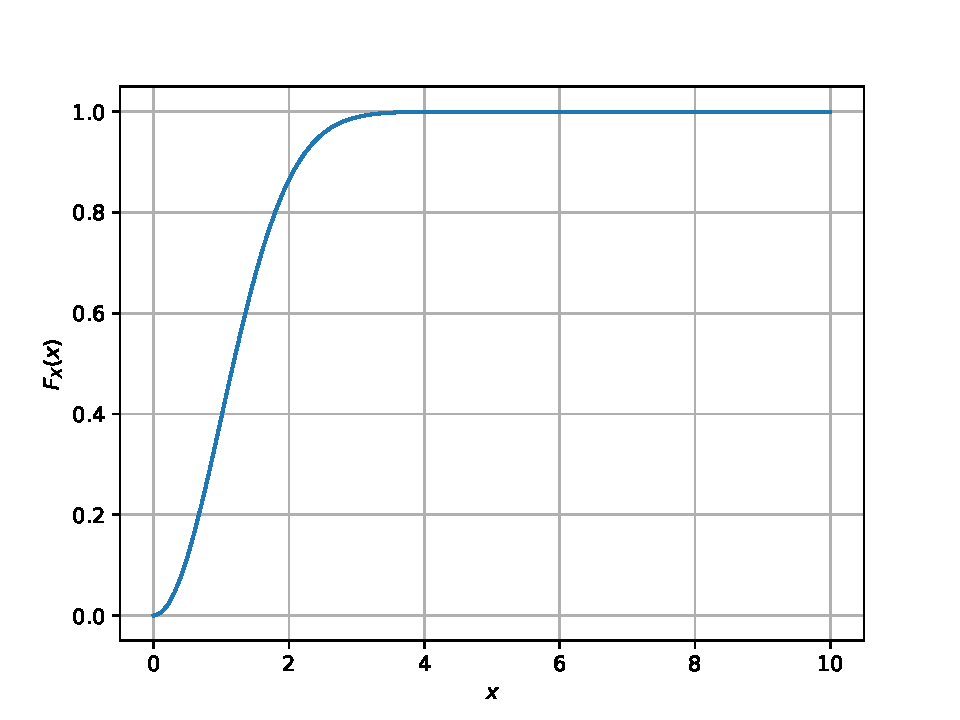
\includegraphics[width=\columnwidth]{/home/mannava/latex/root_cdf.pdf}
\caption{CDF of $A$}
\label{fig:rayleigh_cdf}
\end{figure}
\begin{figure}[H]
\centering
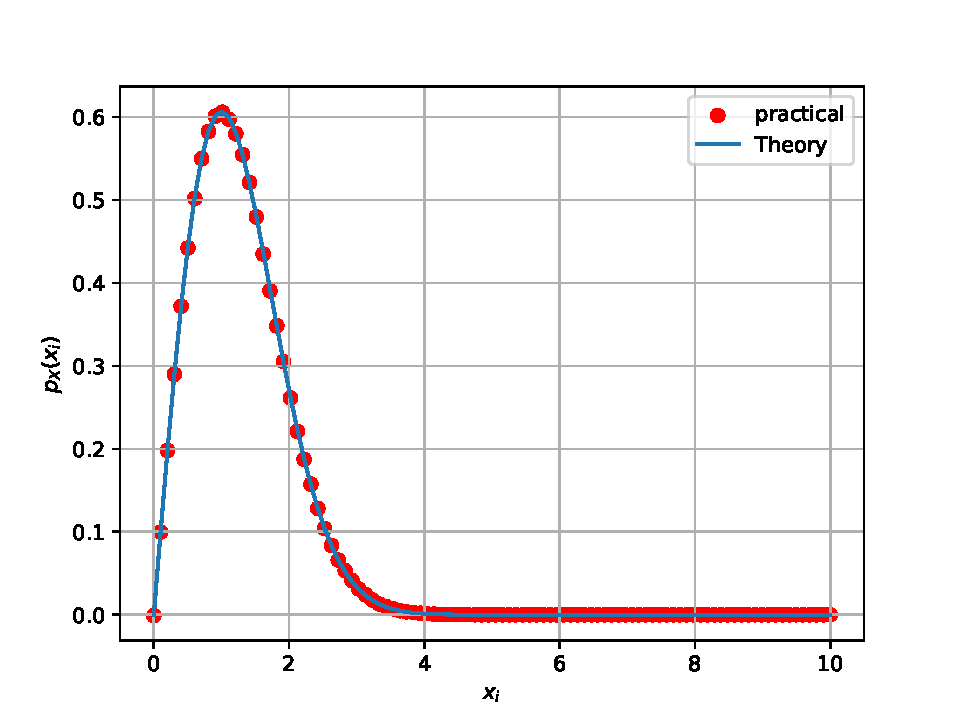
\includegraphics[width=\columnwidth]{/home/mannava/latex/chisq_pdf.pdf}
\caption{PDF of $A$}
\label{fig:rayleigh_pdf}
\end{figure}
%
\end{enumerate}

\section{Conditional Probability}
\begin{enumerate}
\item
\label{ch4_sim}
Plot 
\begin{equation}
P_e = \pr{\hat{X} = -1|X=1}
\end{equation}
%
for 
\begin{equation}
Y = AX+N,
\end{equation}
where $A$ is Raleigh with $E\sbrak{A^2} = \gamma, N \sim \gauss{0}{1}, X \in \brak{-1,1}$ for $0 \le \gamma \le 10$ dB.\\
\solution The blue dots in \figref{fig:bpsk_pe_snr_rayleigh} is the required plot. The below code is used to generate the plot,
\begin{lstlisting}
	https://github.com/Mannava123455/module_2/blob/main/probability/codes/chapter_5/5_1_1.py
\end{lstlisting}
%
\item
Assuming that $N$ is a constant, find an expression for $P_e$.  Call this $P_e(N)$\\
\solution Assuming the decision rule in \eqref{eq:bpsk_decision}, when $N$ is constant, $P_e$ is given by 
\begin{flalign}
	\nonumber
	P_e &= \pr{\hat{X} = -1|X=1}&\\ \nonumber
	&= \pr{Y<0|X=1}&\\ \nonumber
	&= \pr{AX+N<0|X=1}&\\ 
	\label{eq:prob_err_rayleigh_gen}
	&= \pr{A+N<0}&\\ \nonumber
	&= \pr{A<-N}&\\
	\label{eq:prob_err_bpsk_rayleigh_cdf}
	&=
	\begin{cases}
	F_A(-N) & N \ge 0\\
	0 & N < 0
	\end{cases}
\end{flalign}
For a Rayleigh random variable $X$ with $E\sbrak{X^2} = \gamma$, the PDF and CDF are given by
\begin{align}
	\label{eq:rayleigh_pdf}
	p_X(x) &= \frac{2x}{\gamma}\exp\left(-\frac{x^2}{\gamma}\right) \text{ for } x \ge 0\\
	\label{eq:rayleigh_cdf}
	F_X(X) &= 1-\exp\left(-\frac{x^2}{\gamma}\right) \text{ for } x \ge 0
\end{align}
Substituting \eqref{eq:rayleigh_cdf} in \eqref{eq:prob_err_bpsk_rayleigh_cdf},
\begin{equation}
	\label{eq:prob_err_bpsk_rayleigh_fN}
	P_e(N) =
	\begin{cases} 
	1-\exp\left(-\frac{N^2}{\gamma}\right) & N \ge 0\\
	0 & N < 0
	\end{cases}
\end{equation}
%
\item
%
\label{ch4_anal}
For a function $g$,
\begin{equation}
E\sbrak{g(X)} = \int_{-\infty}^{\infty}g(x)p_{X}(x)\, dx
\end{equation}
%
Find $P_e = E\sbrak{P_e(N)}$.\\
\solution Using $P_e(N)$ from \eqref{eq:prob_err_bpsk_rayleigh_fN},
\begin{flalign*}
	P_e &= \int_{-\infty}^{\infty} P_e(x)p_N(x) \,dx&\\
	&= \int_{0}^{\infty} \left(1-e^{-\frac{x^2}{\gamma}}\right)\frac{1}{\sqrt{2\pi}}e^{-\frac{x^2}{2}} \,dx
\end{flalign*}
	
\begin{multline*}
	P_e = \frac{1}{\sqrt{2\pi}}\int_{0}^{\infty} e^{-\frac{x^2}{2}}  \,dx \\ - \frac{1}{\sqrt{2\pi}}\int_{0}^{\infty} \exp\left(-x^2\left(\frac{1}{\gamma}+\frac{1}{2}\right)\right)  \,dx
\end{multline*}
\begin{flalign*}
	P_e &= \frac{1}{2} - \frac{1}{2}\sqrt{\frac{\gamma}{2+\gamma}}
\end{flalign*} 
%
\item
Plot $P_e$ in problems \ref{ch4_sim} and \ref{ch4_anal} on the same graph w.r.t $\gamma$.  Comment.\\
\solution $P_e$ plotted in same graph in \figref{fig:bpsk_pe_snr_rayleigh}. The value of $P_e$ is much higher when the channel %
gain $A$ is Rayleigh distributed than the case where $A$ is a constant (compare with \figref{fig:bpsk_pe_snr}).
\begin{figure}[H]
\centering
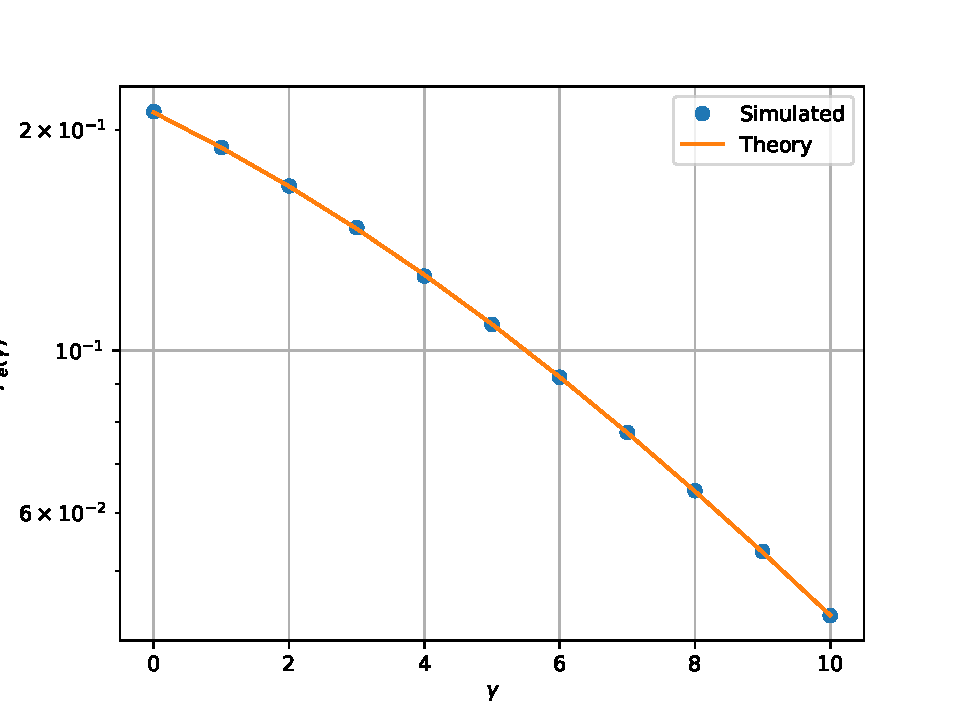
\includegraphics[width=\columnwidth]{/home/mannava/latex/prob_error.pdf}
\caption{$P_e$ versus $\gamma$}
\label{fig:bpsk_pe_snr_rayleigh}
\end{figure}
From \eqref{eq:prob_err_rayleigh_gen}, $P_e$ is given by
\begin{equation}
	P_e = \pr{A+N<0}
\end{equation}
One method of computing \eqref{eq:prob_err_rayleigh_gen} is by finding the PDF of $Z=A+N$ (as the convolution of the individual PDFs of %
$A$ and $N$) and then integrating $p_Z(z)$ from $-\infty$ to $0$. The other method is by first computing $P_e$ for constant $N$ and then finding %
the expectation of $P_e(N)$. Both provide the same result but the computation of integrals is simpler when using the latter method. 

\end{enumerate}

\chapter{Bivariate Random Variables: FSK}
\section{Two Dimensions}
Let 
\begin{equation}
\mbf{y} = A\mbf{x} + \mbf{n},
\end{equation}
where 
\begin{align}
x &\in \brak{\mbf{s}_0,\mbf{s}_1}, 
\mbf{s}_0 = 
\begin{pmatrix}
1 
\\
0
\end{pmatrix},
\mbf{s}_1 = 
\begin{pmatrix}
0 
\\
1
\end{pmatrix}
\\
\mbf{n} &= 
\begin{pmatrix}
n_1
\\
n_2
\end{pmatrix},
n_1,n_2 \sim \gauss{0}{1}.
\end{align}
%
\begin{enumerate}
%%
\item
\label{ch5_fsk}
Plot 
%
\begin{equation}
\mbf{y}|\mbf{s}_0 \text{ and } \mbf{y}|\mbf{s}_1
\end{equation}
%
on the same graph using a scatter plot.\\
\solution 
%
\begin{figure}[H]
\centering
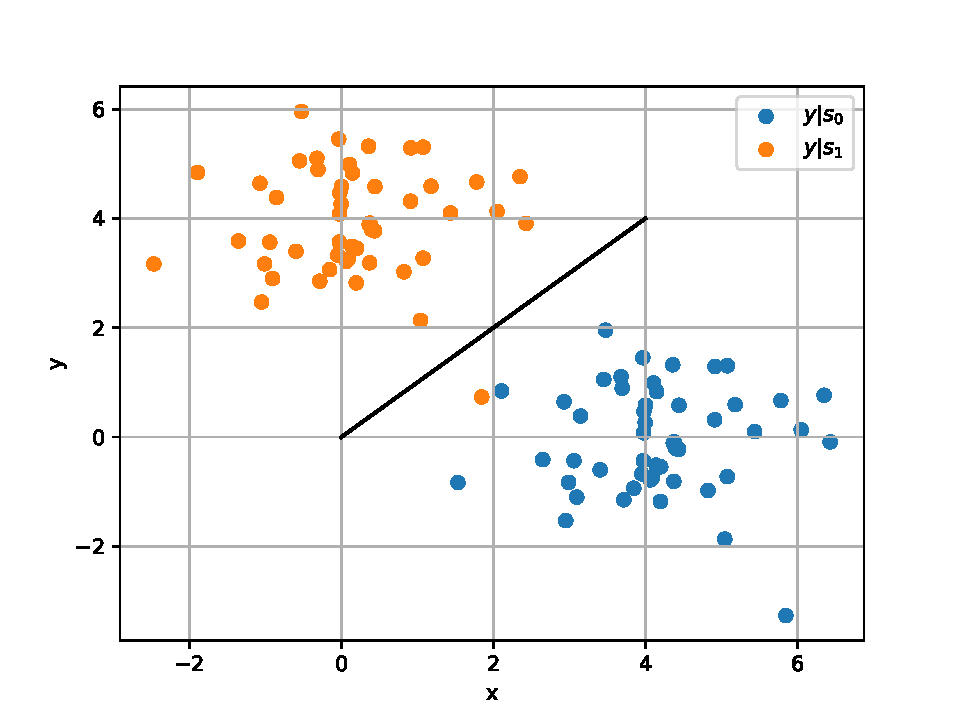
\includegraphics[width=\columnwidth]{/home/mannava/latex/biv_scatter.pdf}
\caption{Scatter plot of $\mbf{y}|\mbf{s}_0$ and $\mbf{y}|\mbf{s}_1$ }
\label{fig:biv_scatter}
\end{figure}

%
\item
For the above problem, find a decision rule for detecting the symbols $\mbf{s}_0 $ and $\mbf{s}_1$.\\
\solution Let $\mbf{y} = \myvec{y_1&y_2}^T$. Then the decision rule is
\begin{equation}
	y_1 \dec{0}{1} y_2
	\label{eq:biv_fsk_decision}
\end{equation}
%
\item
Plot 
\begin{equation} 
P_e = \pr{\hat{\mbf{x}} = \mbf{s}_1|\mbf{x} = \mbf{s}_0}
\label{eq:prob_error_fsk}
\end{equation}
with respect to the SNR from 0 to 10 dB.\\
\solution The blue dots in \figref{fig:biv_pe_snr} are the $P_e$ versus SNR plot. It is generated using the below code,
\begin{lstlisting}
https://github.com/Mannava123455/module_2/blob/main/probability/codes/chapter_5/5_1_3.py
\end{lstlisting}
%
\item
Obtain an expression for $P_e$. Verify this by comparing the theory and simulation plots on the same graph.\\
\solution Using the decision rule from \eqref{eq:biv_fsk_decision},
\begin{align}
	\nonumber
	P_e &= \pr{\hat{\mbf{x}} = \mbf{s}_1|\mbf{x} = \mbf{s}_0}\\\nonumber
	&= \pr{y_1 < y_2|\mbf{x} = \mbf{s}_0}\\\nonumber
	&= \pr{A+n_1 < n_2}\\
	\label{eq:prob_error_fsk_inter}
	&= \pr{n_1-n_2 < -A}
\end{align}
\textbf{Theorem:} The sum of $N$ independant random variables $X_1,X_2,...,X_N$ with $X_i \sim \gauss{\mu_i}{\sigma_i}$ is itself normally distributed %
with $\mu =\sum_{i=1}^n \mu_i$ and $\sigma^2 = \sum_{i=1}^n \sigma_i^2$.\\
Let $Z=n_1-n_2$. From the above theorem, $Z \sim \gauss{0}{\sqrt{2}}$. \eqref{eq:prob_error_fsk_inter} can be further simplified as,
\begin{align*}
	P_e &= \pr{Z < -A}&\\
	&= \pr{Z > A}&\\
	&= \qfunc{\frac{A}{\sqrt{2}}}&\\
	&= \frac{1}{\sqrt{2\pi}}\int_{\frac{A}{\sqrt{2}}}^{\infty} \exp\left(-\frac{x^2}{2}\right)  \,dx 
\end{align*}
\figref{fig:biv_pe_snr} compares the theoretical and simulation plots.

\begin{figure}[H]
\centering
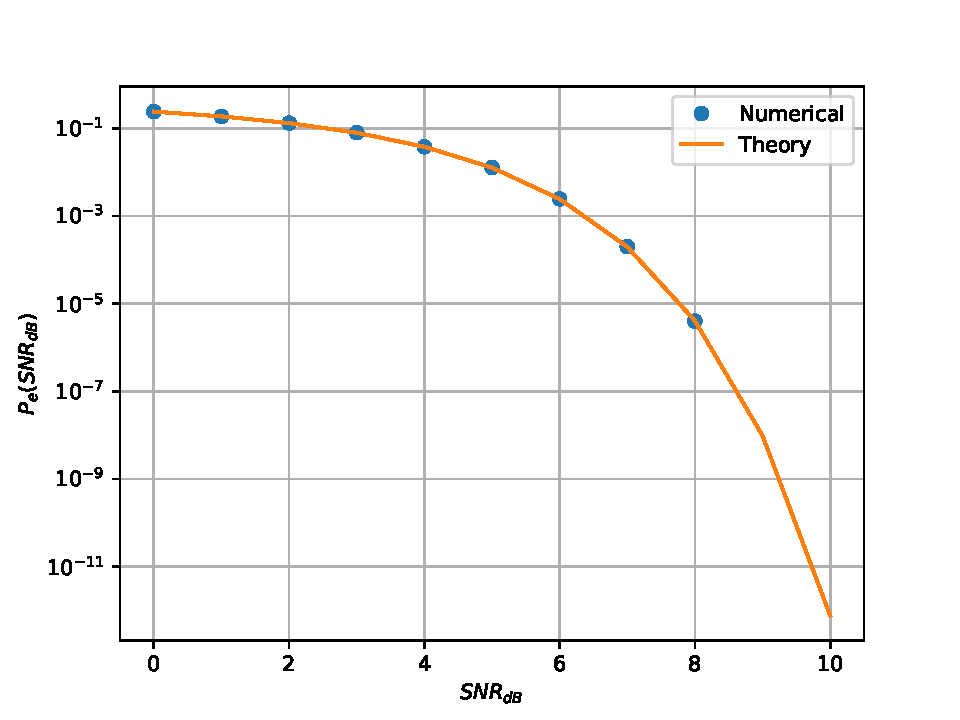
\includegraphics[width=\columnwidth]{/home/mannava/latex/biv_pe_vs_snr.pdf}
\caption{$P_e$ versus SNR plot for FSK}
\label{fig:biv_pe_snr}
\end{figure}
%
\end{enumerate}
\end{document}